\documentclass[tikz,border=6pt]{standalone}
\begin{document}
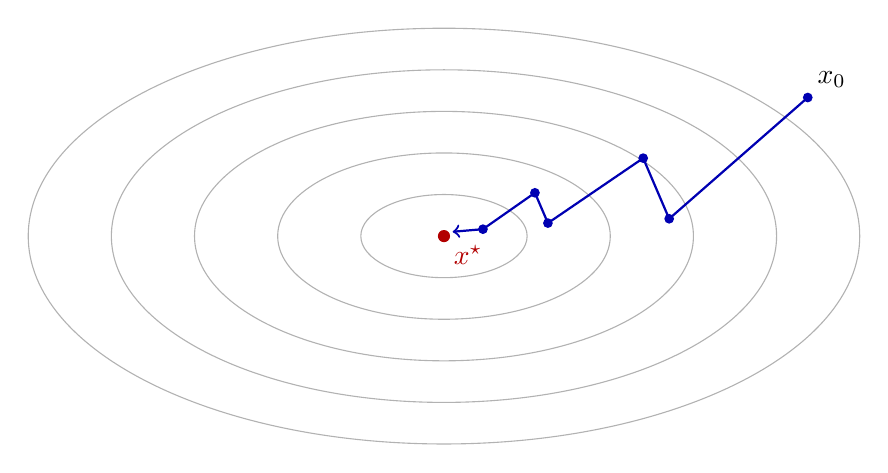
\begin{tikzpicture}[scale=1.1]
  \foreach \r in {0.6,1.2,1.8,2.4,3.0}
    \draw[gray!60] (0,0) ellipse ({\r*1.6} and {\r*0.8});
  \draw[->,thick,blue!70!black] (4.2,1.6) -- (2.6,0.2) -- (2.3,0.9) -- (1.2,0.15) -- (1.05,0.5) -- (0.45,0.08) -- (0.1,0.05);
  \foreach \p in {(4.2,1.6),(2.6,0.2),(2.3,0.9),(1.2,0.15),(1.05,0.5),(0.45,0.08)}
    \fill[blue!70!black] \p circle (1.6pt);
  \fill[red!70!black] (0,0) circle (2pt) node[below right] {$x^\star$};
  \node[above right] at (4.2,1.6) {$x_0$};
\end{tikzpicture}
\end{document}
